%\section{prof.\,Giuseppe Bianchi}
\section{prof.\,Giuseppe Bianchi}
\setcounter{RemarkCounter}{1}
% Prof. Bianchy
\subsection{Remark \theRemarkCounter}
\begin{frame}[allowframebreaks]
    \begin{block}{Remark \theRemarkCounter}
        Did you think about the possibility to include ALUs (Arithmetic and Logic Units) in the
        pipeline in order to further improve programmability? This is (probably, given the very
        obscure and unreliable info available) what the Barefoot PISA chip does (claims to do), and
        would be interesting to compare your architecture with what we can guess the 
        "commercial competitors" do.
    \end{block}
    \begin{exampleblock}{Answer}
        No. All arithmetic and logic operations are known in the time of translation. So,
        there is no need to include complex ALU because all operations are programmed and described in HDL. 
        This approach allows optimization of consumed resources $\rightarrow$ not used operations are not synthesized.
        This is also the advantage of FPGA against ASIC.
    \end{exampleblock}
    
    %\pagebreak
\end{frame}
\stepcounter{RemarkCounter}

\subsection{Remark \theRemarkCounter}
\begin{frame}[allowframebreaks]
    \begin{block}{Remark \theRemarkCounter}
        Somewhat related to the above: P4 includes some instructions which permit some further
        flexibility and programmability also of actions (that's arguably related with the need to
        include ALUs discussed above). Can your approach support "all" the P4
        specifications/instructions or only a subset? If this is the case, can you comment on
        limitations and differences?
    \end{block}
    
    \begin{exampleblock}{Answer}
        The architecture supports a subset of instructions. Packet loopback and packet clone functionality of P4 model are not implemented.
        However, such instructions are mainly the task of infrastructure (around) a P4 pipeline.
        The functionality can be implemented but it can degrade the throughput.
    \end{exampleblock}   
\end{frame}
\stepcounter{RemarkCounter}

\subsection{Remark \theRemarkCounter}
\begin{frame}[allowframebreaks]
    \begin{block}{Remark \theRemarkCounter}
       The SDM approach is not a contribution of this thesis, but is an integral part of your
       approach. Can you please comment on whether you need to adapt the SDM approach, or
       whether you could rely on it with minimal/trivial adaptations? (not fully clear from reading
       the thesis whether you just "used" the SDM approach or needed to further extend it).
    \end{block}
    
    \begin{exampleblock}{Answer}
        %Generally, the SDM approach was known before the P4 and the idea comes from my co-supervisor. 
        My work on HLS allows to extend the SDM with more complex instructions in shorter time.
        This approach can be also used to go beyond a limited set of P4 instructions.
        So, I took results from the previous research and I applied them in my own research.       
%         Generally, the SDM approach was known before the P4 and the idea comes from my co-supervisor. 
%         My work in P4 is based on observations and architectural decisions from the previous research for SDM.
%         So, I adopt the main ideas of general packet processing but I added the flexibility because P4 instructions 
%         are more complex. Moreover, we can use the HLS and go beyond the P4.      
    \end{exampleblock}
\end{frame}
\stepcounter{RemarkCounter}

\subsection{Remark \theRemarkCounter}
\begin{frame}[allowframebreaks]
    \begin{block}{Remark \theRemarkCounter}
         Which challenges and further technical enhancements
         are needed to support stateful processing a la OpenState? It would require a brand new
         design or you believe your architecture can be adapted?        
    \end{block}
    
    \begin{exampleblock}{Answer}
        Current architecture doesn't support the stateful processing a la OpenState. 
        However, I think that the architecture could be extended with OpenState-like processing in Match+Action table 
        $\rightarrow$ we can define the new type of Match+Action table which supports the stateful processing.
    \end{exampleblock}
    
    \pagebreak
    
    \begin{figure}
        \includegraphics[width=\textwidth]{pic/OpenStateConcept}
        \caption{OpenState concept (taken from \url{http://openstate-sdn.org/})}
    \end{figure}
\end{frame}
\stepcounter{RemarkCounter}

%\section{Ing.\,Katar\'{i}na Jelemensk\'{a},\,PhD.}
\section{Ing.\,Katarína Jelemenská,\,PhD.}
\setcounter{RemarkCounter}{1}
% dr. Jelemenska
\subsection{Remark \theRemarkCounter}
\begin{frame}[allowframebreaks]
    \begin{block}{Remark \theRemarkCounter}
        The experiments, discussed in the thesis, are focused mainly on the transformation efficiency
        and the throughput of generated network devices. However, the first thing to prove is the 
        functional correctness. Could you explain, how was the correctness of the transformation 
        process and the generated network devices verified?
    \end{block}
    
    \pagebreak
    
    \begin{exampleblock}{Answer}
        \begin{itemize}
            \fitem \textbf{Block level testing}
                \begin{enumerate}
                    \fitem Functional verification of fundamental idea (for each block) --- manual implementation of first block version + verification environment (similar to \textbf{OVM} - Open Verification Methodology).
                    \fitem Generated block is connected instead of the manual implementation.
                \end{enumerate}
            \fitem \textbf{Integration testing}
                \begin{enumerate}
                    \fitem Manual implementation of functional verification environment for complex (generated) pipelines.
                    \fitem Verification of different use-cases in real environment against the Spirent Test device.
                \end{enumerate}
        \end{itemize}
        
        However, I know that this is not sufficient and it drives me to design the automatic test environment.
    \end{exampleblock}
    
    \pagebreak
    \begin{figure}
        \vspace*{0pt}
        \centering
        \includegraphics[width=0.99\textwidth]{pic/p4-testbed}
    \end{figure}
      
\end{frame}
\stepcounter{RemarkCounter}

\subsection{Remark \theRemarkCounter}
\begin{frame} %[allowframebreaks]
    \begin{block}{Remark \theRemarkCounter}
        In section 4.1.3 a possibility of P4 program optimization is discussed. It is clear that P4
        program has to be designed manually. However, based on the provided optimization example it
        looks like it could be then optimized automatically. Why is it not possible?
    \end{block}
    
    \begin{exampleblock}{Answer}
        The automation of such optimization is not the part of my thesis because we found the only one specific example (TCP/UDP). 
%        The automation of such optimization wasn't part of my thesis because we identified one 
%        specific example (TCP/UDP).
    \end{exampleblock}

\end{frame}
\stepcounter{RemarkCounter}

\subsection{Remark \theRemarkCounter}
\begin{frame}[allowframebreaks]
    \begin{block}{Remark \theRemarkCounter}
            In most of the related authors publications one of the co-author is Viktor Puš.
            For example the papers A.1 and A.2 resemble the summary of this thesis. 
            Could you strictly distinguish the contribution of the two authors?
    \end{block}
    
    \begin{exampleblock}{Answer}
        Dr.\,Puš came with the main idea of modular parser and he also provided the first manual implementation. The rest of presented work (in the thesis) is mine.
    \end{exampleblock}  
     %\pagebreak
\end{frame}
\stepcounter{RemarkCounter}

%\section{Dr.\,Alistair McEwan}
\section{Dr.\,Alistair McEwan}
\setcounter{RemarkCounter}{1}
%dr. McEwan
\subsection{Remark \theRemarkCounter}
\begin{frame}[allowframebreaks]
    \begin{block}{Remark \theRemarkCounter}
        Chapter 2 discussed the benefits and drawbacks of a variety of languages used in this study,
        and others. However the evaluation of these languages seems rather subjective---based either
        on the authors view, or on the view of those whose work he cites. An example of this is
        Handel-C: the language was intended to make reconfigurable hardware accessible to software
        engineers, rather than focus on performance (and the reviewer published some work in this
        area, specifically relating to the efficiency of CAM architectures on FPGA-based network
        architectures). How might an evaluation of languages in this area be made more objective?
    \end{block}
    
    \pagebreak
    
    \begin{exampleblock}{Answer}
        Reviewer is right that evaluation of discussed languages are based on my and others views. 
        We can do the following for more objective evaluation:
        \begin{enumerate}
            \fitem Obtain a set of problems, languages and developers.
            \fitem Let each developer implements the set of problems in given languages.
            \fitem Finally, we compare parameters of synthesized designs like frequency, consumed resources and time required for development.
        \end{enumerate}
    \end{exampleblock}
\end{frame}
\stepcounter{RemarkCounter}

\subsection{Remark \theRemarkCounter}
\begin{frame}[allowframebreaks]
    \begin{block}{Remark \theRemarkCounter}
        A corollary of the above question concerns the use of T-CAMs in chapter 5. What are the
        trade-offs between a single cycle lookup, hardware costs, latency, and overall throughput?
        It would seem intuitive that a significant amount of actions implemented in a T-CAM could
        considerably skew some of these results.
    \end{block}
    
    \pagebreak
    
    \begin{table}
        \centering
        \footnotesize
        \begin{tabular}{|c|c||c|c|c|}
        	\hline
        	\T\textbf{Search time\,[\# clk.]} & \textbf{\# Entries} & \textbf{LUT} & \textbf{Regs.} & \textbf{Freq.\,[MHz]} \\ \hline\hline
        	      \T\multirow{4}{*}{1}        &         64          &     2015     &      343       &        399.52         \\
        	                                  &         128         &     3807     &      409       &        294.55         \\
        	                                  &         256         &     7395     &      537       &        293.08         \\
        	                                  &         512         &    14587     &      795       &        291.63         \\ \hline
        	                %                 &        1024         &    29143     &      1311      &        291.61         \\
        	                %                 &        2048         &    58049     &      2338      &        291.63         \\
        	      \T\multirow{4}{*}{2}        &         64          &     1384     &      345       &        363.63         \\
        	                                  &         128         &     2551     &      410       &        361.40         \\
        	                                  &         256         &     4608     &      539       &        360.62         \\
        	                                  &         512         &     8939     &      796       &        358.42         \\ \hline
        	                %                 &        1024         &    17667     &      1309      &        356.25         \\
        	                %                 &        2048         &    35339     &      2334      &        366.03         \\
        	      \T\multirow{4}{*}{4}        &         64          &     943      &      346       &        365.23         \\
        	                                  &         128         &     1639     &      411       &        362.97         \\
        	                                  &         256         &     3035     &      540       &        360.75         \\
        	                                  &         512         &     5546     &      797       &        359.97         \\ \hline
        \end{tabular}
        \caption{Required resources of used TCAM (132 bit search key)}
     \end{table}
     % Insert the enumeration to minipage because we want to move with it up
     \vspace*{-1px}
     \begin{minipage}{\textwidth}
          \begin{itemize}
              \fitem LUT based implementation
              \fitem Xilinx Vivado 2016.3, Virtex\,7 580thcg1931-2 FPGA
              \fitem Frequency and resources are after synthesis
          \end{itemize}
     \end{minipage}
\end{frame}
\stepcounter{RemarkCounter}

\subsection{Remark \theRemarkCounter}
\begin{frame}[allowframebreaks]
    \begin{block}{Remark \theRemarkCounter}
       The techniques in chapters 4 and 5 draw on a translation from P4 to VHDL. However to the
       best of my knowledge, this translation only seems to be presented in terms of some examples.
       This may not be the most robust approach: it is not clear exactly how this is defined in the
       tools, and whether or not the translation is a simple syntactic one or a deeper semantic one.
       What are the implications of this, and if a deeper semantic integration---such as via abstract
       data types---is not preferable, why is this the case?     
    \end{block}
    
    \begin{exampleblock}{Answer}
        The deeper semantic for translation of P4 to VHDL is not given in my thesis. The main characteristic of the problem is:
        \begin{itemize}
            \fitem The semantic of VHDL and P4 is a set of narrative rules.
            \fitem The semantic of P4 and VHDL is not formally defined in their standards.
            \fitem The target architecture (know-how) of network device is given and it is designed based on my experiences with high-speed network processing in FPGA.
        \end{itemize}
        
        I provided a mapping from P4 to VHDL based on target architecture and sets of narrative rules.
    \end{exampleblock}
    
    \begin{figure}
        \centering
        \includegraphics[scale=0.709]{pic/p4-to-vhdl-relations}
    \end{figure}
\end{frame}
\stepcounter{RemarkCounter}

\subsection{Remark \theRemarkCounter}
\begin{frame}[allowframebreaks]
    \begin{block}{Remark \theRemarkCounter}
       In the case studies, the author talks about the effort in developing bespoke hardware in
       VHDL to be approximately twice as costly in terms of time as the software defined C++
       approach. Is this a result that one should care about, or is it in fact a result that demonstrates
       the two solutions are broadly similar in terms of effort? Perhaps this could also be considered
       relative to higher level hardware descriptions?
    \end{block}
    
    \begin{exampleblock}{Answer}
        It matters on requirements and priorities (small chip area, time of development, and so on).
        I experiment with HLS in the case of SDM. In such case, all used instructions were relatively 
        simple and they were coded two times faster in higher language C/C++ (easier updates and debugging, faster deployment).
    \end{exampleblock}
\end{frame}
\stepcounter{RemarkCounter}

\subsection{Remark \theRemarkCounter}
\begin{frame}[allowframebreaks]
    \begin{block}{Remark \theRemarkCounter}
       A final question which I have not really been able to ascertain from the results and the
       conclusions drawn from them: where does the author feel the weaknesses of his technique and
       architecture lie? Algorithmic complexity of parsing seems fine, hardware costs of the resulting
       implementations are broadly acceptable, performance results meet their requirements, and
       hand-coding of optimizations seems perfectly tractable!
    \end{block}
    
    \begin{exampleblock}{Answer}
         \begin{itemize}
             \fitem Deparser does not support the full throughput.
             \fitem Packet loopback/clone instructions are not supported.
             \fitem The tool for easy programming of rules is not available.
             \fitem Scalability for smaller data widths (architecture is optimized for wide data paths).
         \end{itemize} 
    \end{exampleblock}
\end{frame}